\subsection{Circuito I: VFA-VFA}
\hspace{1mm} El amplificador operacional que se implementa para el circuito propuesto es el LM328 para el circuito propuesto.  integrados que se utilizan para el amplificador VFA es el LM324 cuyas especificaciones se detallan a continuación.

\begin{itemize}[itemsep=1pt]
    \item \(A_{d0}=100~dB\)
    \item \(F_T=1~MHz\)
    \item \(F_1=10~Hz\)
    \item \(F_2=5.06~MHz\)
\end{itemize}

\bigskip
\hspace{1mm} Seguidamente, se calculará la ganancia del circuito considerando el segundo AO como ideal. Para ello, se deberán calcular las ganancias de lazo abierto \(Ad(s)\), ganancia de lazo \(T(s)\) y ganancia de lazo cerrado \(Avf(s)\). Con todos estos datos se procederá a compensar el amplificador compuesto para lograr una máxima planicidad de módulo.

\begin{figure}[!h]
    \centering
    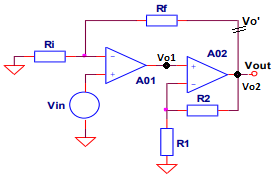
\includegraphics[scale=1.2]{Imagenes/Punto1LazoCerradoVoP.png}
    \caption{Amplificador compuesto VFA-VFA}
\end{figure}

\hspace{1mm} Se obtiene la ganancia de lazo abierto. Esta misma es la relación entre la tensión de salida y la tensión de entrada.

\begin{equation}
    Av(s) = \frac{V_{out}}{V_{in}}
\end{equation}

\bigskip
\hspace{1mm} Se obtienen las expresiones de las tensiones \(V_{o1}\) y \(V_{o2}\).

\begin{equation}
    V_{o1} = Ad(s)\cdot V_{in} 
\end{equation}

\begin{equation}
     V_{o2} =V_{out}= V_{o1}\cdot \Bigl(1+\frac{R_2}{R_1}\Bigl)
\end{equation}

\begin{equation}
    V_{o2} =V_{out}= Ad(s) \cdot V_{in} \cdot \Bigl(1+\frac{R_2}{R_1}\Bigl)
\end{equation}

\hspace{1mm} La relación entre la salida y la entrada da como resultado la ganancia de lazo abierto.

\begin{equation}
    \boxed{
    Av(s) = Ad(s)\cdot \Bigl(1+\frac{R_2}{R_1}\Bigl)
    }
\end{equation}

\bigskip
\hspace{1mm} Luego, se calcula la ganancia de lazo T.

\bigskip
    \[T(s) = \frac{V_{out}}{V_{out'}}|_{V_{in}=0}\]

\hspace{1mm} Entonces.
\[V_{o1}= Ad(v^+-v^-)\]
\[V_{o1}= Ad.\Bigl(0V-V_{o}'\frac{R_i}{R_i+R_f}\Bigl)=-Ad.V_{o}'\Bigl(\frac{R_i}{R_f}+1\Bigl)\]
\begin{equation}\label{eq:primera_etapa} 
\boxed{V_{o1} = -Ad.V_{o}'\Bigl(\frac{R_i}{R_f}+1\Bigl)}
\end{equation}

\bigskip
\hspace{1mm} Luego, \(V_{out}\)  ha sido calculado para la ganancia de lazo abierto.

\begin{equation}
    V_{out}= V_{o1}\cdot \Bigl(1+\frac{R_2}{R_1}\Bigl)
\end{equation}

\hspace{1mm} Por lo tanto, 

\begin{equation}
    \boxed{
      T(s) = -Ad(s)\cdot \Bigl(\frac{R_2}{R_1}+1\Bigl)\cdot \Bigl(\frac{R_i}{R_f}+1\Bigl)
    }
\end{equation}
  
\bigskip
\hspace{1mm} Se tiene que la ganancia de lazo cerrado es:

\begin{equation}
    Avf(s) = \frac{Av(s)}{1-T}
\end{equation}

\begin{equation}
      Avf(s) = \frac{Ad(s)\cdot \Bigl(\frac{R_2}{R_1}+1\Bigl)}{1+Ad(s)\cdot \Bigl(1+\frac{R_2}{R_1}\Bigl)\cdot \Bigl(\frac{R_i}{R_f}+1\Bigl)}
\end{equation}

\bigskip
\hspace{1mm} Considerando la ganancia \(Ad(s)\) tiende a infinito, se simplifican los cálculos referidos a la ganancia de lazo cerrado.

\bigskip
\begin{equation}
      Avf(s) = \lim_{x\to\infty} \frac{Ad(s)\cdot (\frac{R_2}{R_1}+1)}{1+Ad(s)\cdot (1+\frac{R_2}{R_1})\cdot \Bigl(\frac{R_i}{R_f}+1\Bigl)}
\end{equation}
\begin{equation}
    \boxed{
        Avf(s)=\Bigl(\frac{R_f}{R_i}+1\Bigl) 
    }
\end{equation}

\bigskip
\hspace{1mm} El requerimiento con respecto a la ganancia es que debe ser \(Avf(s)=20~dB\). Con este dato, se obtiene la relación entre las resistencias \(R_i\) y \(R_f\).
\begin{equation}
    Avf(s)=20~dB
\end{equation}
\begin{equation}
    20~dB=20\cdot\log{(Avf)}
\end{equation}
\begin{equation}
    \log{(Avf)}=\frac{20~dB}{20}
\end{equation}
\begin{equation}
    \log{(Avf)}=1
\end{equation}
\begin{equation}
    Avf=10
\end{equation}
\begin{equation}
    \Bigl(\frac{R_f}{R_i}+1\Bigl)=10
\end{equation}
\bigskip
\hspace{1mm} Despejando la relación de resistencias.
\bigskip
\begin{equation}
    \frac{R_f}{R_i} = 9 \hspace{7mm} R_f=R_i \cdot 9
\end{equation}
\begin{equation}
    R_f=R_i \cdot 9
\end{equation}

\bigskip
\hspace{1mm} Se colocan valores arbitrarios de resistencias que cumplan con la relación anteriormente hallada.

\begin{equation}
    \boxed{
        R_i=10~k\Omega \hspace{3mm} , R_f=90~k\Omega
    }
\end{equation}

\bigskip

\hspace{1mm} Se realiza la simulación en el software Octave de la función transferencia del amplificador operacional.

\begin{lstlisting}
clear all; close all; clc

%Include the pakage control and define 's' as Laplace variable
%pkg load control;
s= tf('s');

%Function Transfer
FT= (100^3)/((1+(s/(10*2*pi)))*(1+(s/(2*pi*(5.06e+6)))));

%Display Bode Plot
bode(FT);
grid on; 
\end{lstlisting}
\bigskip

\hspace{1mm}  Se realiza la gráfica de Bode de la función transferencia de lazo abierto del amplificador operacional (LM324) implementando el software Matlab. El amplificador operacional anteriormente nombrado tiene un polo en \(10~Hz\) y otro en \(5.06~MHz\).

\begin{figure}[h!]
  \centering
    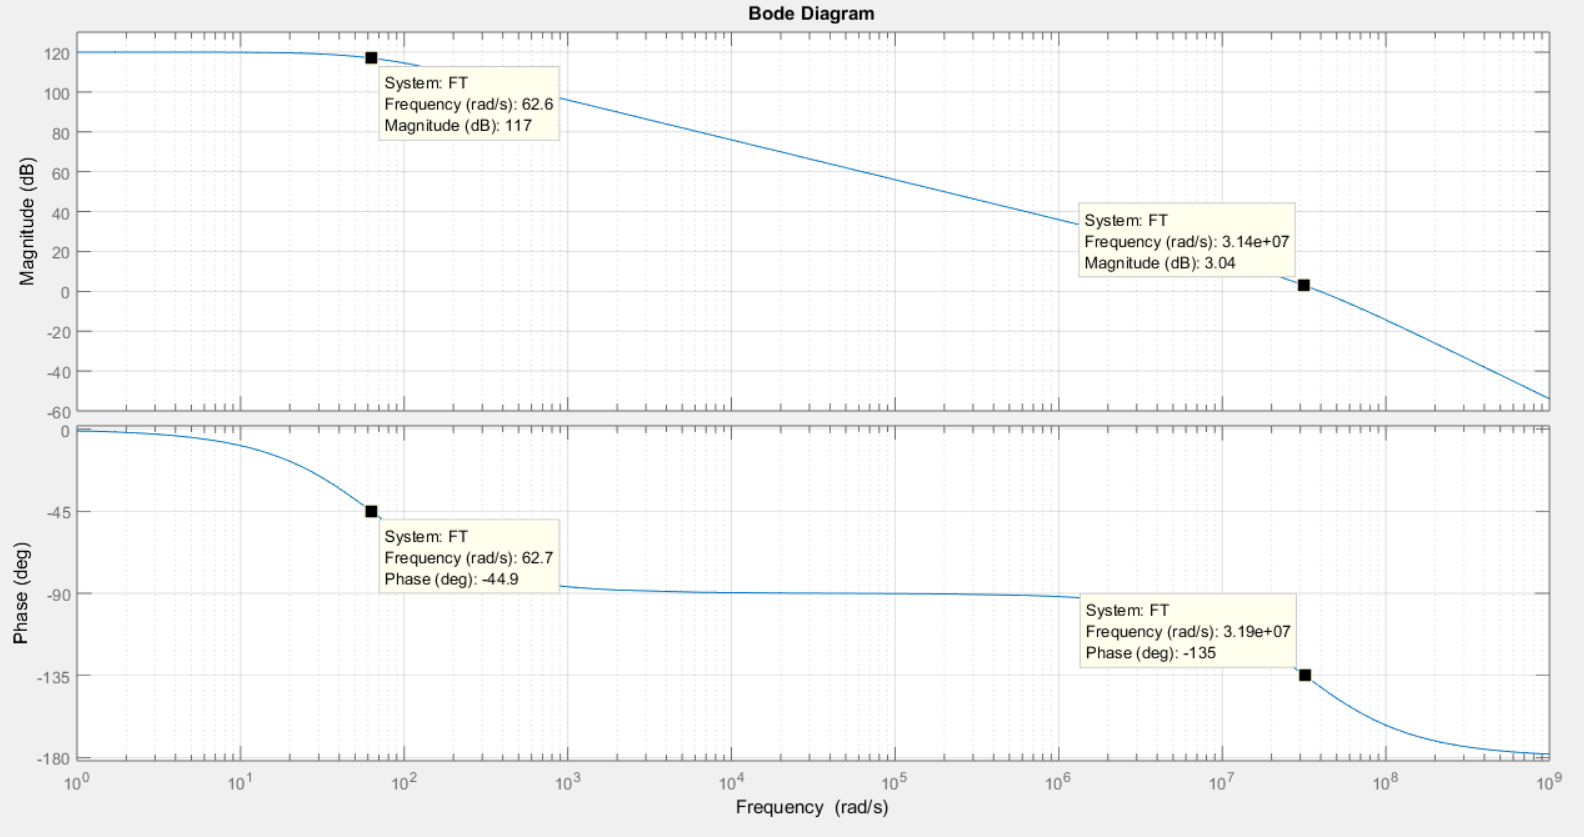
\includegraphics[scale=0.5]{VFA VFA/Imágenes/Circuito 1 - Bode Plot.png}
    \caption{Diagrama de Bode del amplificador lazo abierto}
\end{figure}

\bigskip
\hspace{1mm} Se tiene que uno de los requerimientos es que se debe tener máxima planicidad de módulo \(M\varphi =65°\).  A lazo cerrado se encuentra un polo en \(f_g\) el cual esta relacionado con la ganancia del amplificador \(A_{o2}\).
\bigskip

\hspace{1mm} Se considera que el amplificador \(A_{o2}\) es ideal. determinando a continuación la fórmula del margen de fase de la cual se despejó el polo \( 
f_g \)
 
\begin{equation}
    M \varphi = 360^o - 180^o - arctg \left( \frac{f_g}{f_1} \right) - arctg \left( \frac{f_g}{f_2} \right) = 65^o
\end{equation}
\begin{equation}
    M \varphi = 180^o - arctg \left( \frac{f_g}{f_1} \right) - arctg \left( \frac{f_g}{f_2} \right) = 65,5^o
\end{equation}
\begin{equation}
    115^o = arctg \left( \frac{f_g}{f_1} \right) + arctg \left( \frac{f_g}{f_2} \right)
\end{equation}
\begin{equation}
    \boxed{
    f_g = 2,36~MHz
    }
\end{equation}
\bigskip
\hspace{1mm} Se determinó la ganancia a lazo cerrado del amplificador \(A_{O2}\) ideal de la siguiente manera. Considerar que la ganacia de lazo cerrado ideal fue dada en la consigna y es la siguiente \((Avfi=20~dB)\).


\begin{equation}
    Avf_{2i}=\frac{Avfi \cdot \omega_{gi}}{Ad_0 \cdot \omega_1} = 27~dB
\end{equation}

\bigskip
\hspace{1mm} Siendo \( \omega _{gi} = 2\pi f_g \)
y, \( \omega _1 \) y  \(\omega _2\) la frecuencia del primer y segundo polo respectivamente, especificada en frecuencia angular.


\bigskip
\hspace{1mm} Este valor de ganancia se utilizó para obtener la ganancia del amplificador compuesto.

\begin{equation}
    Av_{comp}=Ad0\cdot Avf_{2i}=100~dB \cdot 27~dB
\end{equation}

\begin{equation}
    \boxed{
    Av_{comp} = 127~dB
    }
\end{equation}

\bigskip

\hspace{1mm} Se diseña la función de transferencia de lazo cerrado del amplificador compuesto \(A_{vf_{comp}}\). Se determina la ganancia de ruido global \(K_{global}\).

\[20~dB= 20 \log(A_{vf_{comp}})\]
\[\log(A_{vf_{comp}})=\frac{20~dB}{20}\]
\[A_{vf_{comp}}=10^{1}\]
\[A_{vf_{comp}}=10\]
\begin{equation}
    K_{global} = \frac{1}{A_{vf_{comp}}} = \frac{1}{10}
\end{equation}
\begin{equation}
    \boxed{
    K_{global} = 0.1
    }
\end{equation}

\bigskip
\hspace{1mm} Se resolvió así la función de transferencia mencionada.

\begin{equation}
    FtAvf (comp) = \frac{Ad_0 \cdot Avf_{2i} \cdot \omega_1 \cdot \omega_2}{s^2 + s \cdot (\omega_1 + \omega_2) + (\omega_1 \cdot \omega_2 + K (global) \cdot Ad_0 \cdot Avf_{2i} \cdot \omega_1 \cdot \omega_2)}
\end{equation}

\begin{equation}
    FtAvf (comp) = \frac{Ad_0 \cdot Avf_{2i} \cdot \omega_1 \cdot \omega_2}{s^2 + s \cdot (\omega_1 + \omega_2) + (\omega_1 \cdot \omega_2 + K (global) \cdot Ad_0 \cdot Avf_{2i} \cdot \omega_1 \cdot \omega_2)}
\end{equation}

\begin{equation}
    A_{vf_{comp}}(s) = \frac{4,714 \cdot 10^{15}}{s^2 + 3,179 \cdot 10^7 \cdot s + 4,713 \cdot 10^{14}}
\end{equation}

\bigskip
\hspace{1mm} Dicha función transferencia se compara con la expresión de un sistema de segundo orden:
\begin{equation}
    A_{v}(s) = \frac{\omega _p^2}{s^2 + s \frac{\omega _p}{Q_p } + \omega_p^2}
\end{equation}  
\bigskip
\hspace{1mm} Se igualan las ecuaciones y se determinan los siguientes parámetros:
\begin{equation}
    \omega _p ^2 = 4,713 \times 10^{14} \Longrightarrow \omega_p =\sqrt{4,713 \times 10^{14}} 
\end{equation}
\begin{equation}
    \boxed{
        \omega_p = 21,7 \cdot 10^6 \space \frac{rad}{seg} 
    }
\end{equation}
\bigskip
\hspace{1mm} Entonces, la frecuencia del polo compensado es:

\begin{equation}
    f_p = \frac{\omega_p}{2\pi}=\frac{21,7 \cdot 10^6 \frac{rad}{seg}}{2\pi}
\end{equation}

\begin{equation}
    f_p = 3,45\cdot 10^6 \space Hz= 3,45\space MHz
\end{equation}
\begin{equation}
    \boxed{
    f_p = 3,45\space MHz
    }
\end{equation}

\bigskip
\hspace{1mm} Se comprueba que \( Q_p \).

\begin{equation}
    3,179 \cdot 10^7 \frac{rad}{seg} = \frac{\omega_p}{Q_p} 
\end{equation}
\begin{equation}
    Q_p = \frac{\omega_p}{3,179 \cdot 10^7} = \frac{21,7 \cdot 10^6 \frac{rad}{seg}}{3,179 \cdot 10^7} = 0,696 \approx 0,7
\end{equation}

\begin{equation}
    \boxed{
    Q_p = 0,7
    }
\end{equation}


\begin{figure}[!h]
    \centering
    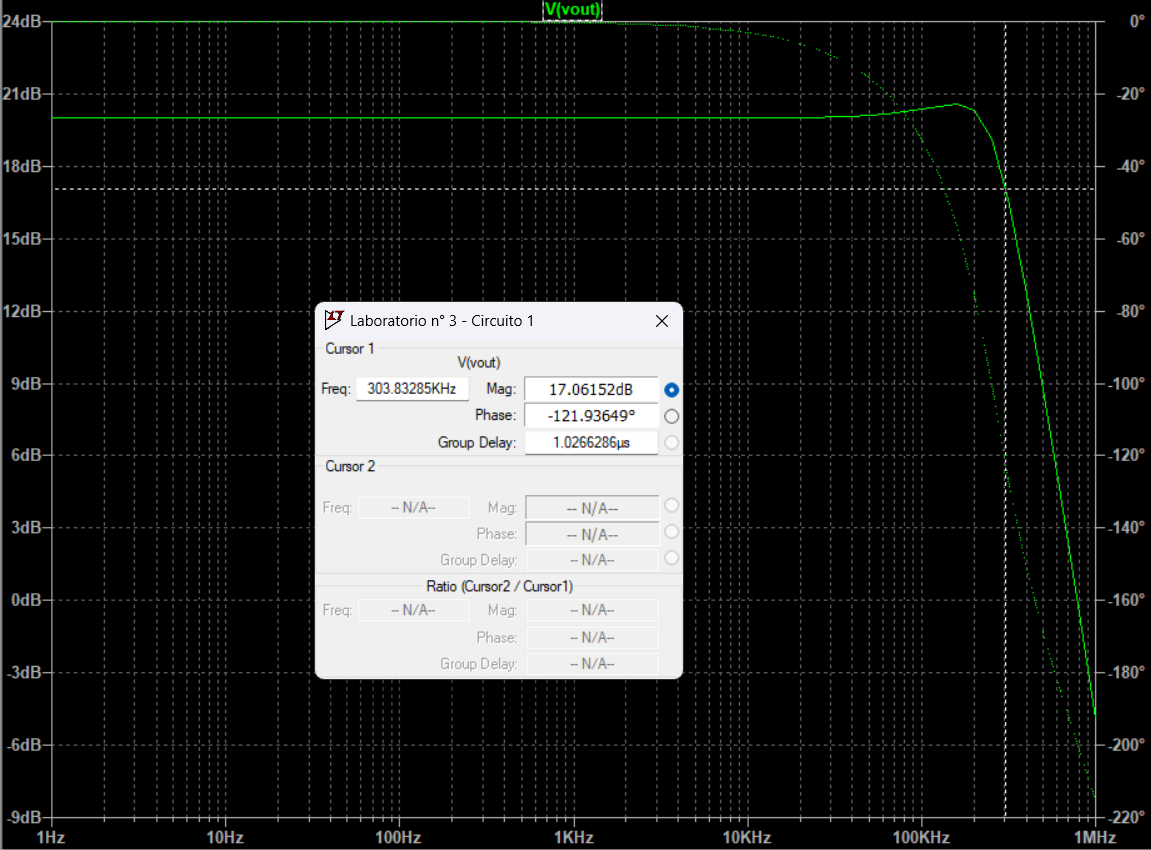
\includegraphics[scale=0.7]{VFA VFA/Imágenes/VFA VFA Sistema realimentado.png}
    \caption{Diagrama de Bode del amplificador compuesto}
\end{figure}

\hspace{1mm} Como la ganancia de lazo cerrado es igual a \(Avf_2=27~dB\) y, por lo tanto, la ganancia del amplificador compuesto a lazo abierto resulta ser \(127~dB\). Con estos valores, se puede calcular el valor del polo \(f_g\).

\begin{equation}
    \frac{127~dB-20~dB}{log(10)-log(f_g)}=-20~dB/dec
\end{equation}

\bigskip
\hspace{1mm} Se despeja \(f_g\), y se obtiene:

\begin{equation}
\boxed{
    f_g=2.2~MHz
}
\end{equation}
